
\label{elektronika}

\subsubsection*{Datasheet}

{\bf Datasheet} \index{datasheet} je dokument, ve kterém jsou detailně popsány vlastnosti a možnosti dané elektronické součástky.
Každá součástka má svůj datasheet. 

Datasheet pro každou součástku je možné najít na webu, například na stránce \url{www.datasheetcatalog.com}
nebo na stránkách výrobce/prodejce součástky. 
Všechny datasheety jsou anglicky.  

\subsubsection*{Nepájivé kontaktní pole} \label{nepajive_pole} \index{Nepájivé kontaktní pole}

 \href{https://cs.wikipedia.org/wiki/Nep\%C3\%A1jiv\%C3\%A9_pole}{Nepájivé kontaktní pole}
  slouží pro první rychlé zapojení součástek do vytvářeného obvodu.
 Je to deska s maticí otvorů, které jsou vždy po pěti propojené. Do těchto otvorů zasunujete vývody součástek a podle potřeby je spojujete pomocí drátků. Díky tomu nemusíte pracovat s páječkou, a zároveň je zapojený obvod snadno rozebiratelný, takže můžete zapojení sestavovat, testovat, upravovvat a opět rozmontovávat. Po stranách jsou navíc dlouhé lišty otvorů určené pro přivedení napájení. 


\section{Jednoduché součástky} 


\subsection{Rezistor} \label{rezistor}

{\bf Rezistor}  \index{rezistor} nebo také odpor\footnote{Správně se součástce říká rezistor, odpor je její vlastnost.
	 Ale mnoho lidí používá pro označení součástky slovo odpor.} je součástka, která klade elektrickému proudu  určitý odpor neboli ho omezuje. 
	Toho se používá jako ochrana před zničením čipu nebo jeho části. Odpor se značí $R$. Jednotkou odporu je 1~Ohm, značka $\Omega$. 

 Dva rezistory (nebo jiné součástky) mohou být zapojeny buď 
 {\bf sériově}  \label{seriove}
 (tj. za sebou) nebo {\bf paralelně} (tj. vedle sebe), viz obrázek \ref{fig:rezistory}. 
\index{zapojení!sériové}\index{sériové!zapojení}\index{zapojení!paralelní}
\index{paralelní!zapojení} 

\begin{figure}[h]
	\begin{center}
	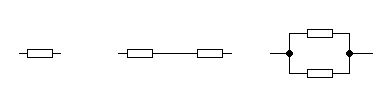
\includegraphics[width=0.5\textwidth]{soubory/rezistory.jpg}		
	\end{center}
	\caption{ vlevo: značka rezistoru, uprostřed: rezistory zapojené sériově, vpravo: rezistory zapojené paralelně} 
	\label{fig:rezistory}
\end{figure}

Speciální roli v čipu mají interní\footnote{vnitřní, zabudované} tzv. 
\href{https://maly.gitbooks.io/hradla-volty-jednocipy/13_jak_naucit_kamen_pocitat/139_pull_up_apulldown.html}{pull-up a pull-down} rezistory. 
%podrobněji v \cite[strana~49]{hr}. 


\subsection{Kondenzátor}

{\bf Kondenzátor}\index{kondenzátor} je součástka, která uchovává elektrický náboj. 
Jeho hlavní vlastností je kapacita. Jednotkou kapacity je Farad, značka F. 
V~praxi se používají násobky jako mikrofarad ($\mu$F), nanofarad (nF) a~pikofarad\footnote{Mikrofarad je miliontina faradu,
	 nanofarad je tisíckrát menší a~pikofarad milionkrát menší než mikrofarad.} (pF). 
	Kondenzátory se nabíjí a~vybíjí různě rychle a~mají různou kapacitu. Keramické kondenzátory 
\index{kondenzátor!keramický}  mají nejmenší kapacitu(pF, nF) a~jejich nabití a vybití je nejrychlejší, tantalové  
\index{kondenzátor!tantalový} mívají kapacitu okolo pár $\mu$F a~jejich nabití a vybití je pomalejší a~nejpomalejší 
jsou elektrolytické\index{kondenzátor!elektrolytický} s~kapacitou stovek až tisíců $\mu$F. 
U~tantalových a~elektrolytických kondenzátorů musíme dát pozor na polaritu, tj. kam připojujeme + a~kam -. 
Další důležitý údaj je maximální hodnota napětí, kterou kondenzátor snese. 

Kondenzátory dokážou eliminovat napěťové špičky, které by jinak znemožnily provoz řídící desky. 
Proto je připojujeme paralelně ke zdrojům napěťových špiček (motory, serva).
%todo napsat líp 

\subsection{Dioda}

{\bf Dioda} \index{dioda} je součástka, která usměrňuje elektrický proud. 
To znamená, že pokud ji zapojíme do elektrického obvodu, tak zajistí, že proud bude téct pouze jedním směrem. 
Proto budeme diodu používat jako ochranu 
proti tzv. {\bf přepólování}\index{přepolóvání!ochrana}\index{ochrana!přepolóvání}
 -- chybnému zapojení baterie nebo součástky do obvodu, které obvykle vede ke zničení součástky. 
U~samotné diody také záleží na polaritě, tj. při jejím zapojení musíme dávat pozor, kde má kladný pól a~kde záporný. 

Na diodě vzniká úbytek napětí, se kterým musíme počítat při návrhu obvodu. 
Tak například pokud připojím na diodu s~úbytkem napětí 0,6~V připojím 12~V, tak za diodou bude napětí 11,4~V. 

Ze začátku nám bude stačit, pokud budeme používat diody  
 \hyperlink{1N4148}{1N4148} a 
 \hyperlink{1N4007}{1N4007}.
   
\subsection{LED}

\hypertarget{LED}{}  
{\bf LED}\footnote{Light emitting diode -- světlo vysílající dioda}
\index{LED}\index{dioda!LED}\index{LED!dioda}   
je součástka, která není primárně určená k~usměrnění proudu, ale k~signalizaci, zda obvodem protéká proud.
K~LED se vždy musí připojit  \hyperref[vypocet_rezistor]{vhodný} rezistor. 

\subsection{Tranzistor} \label{tranzistor}

{\bf Tranzistor}\index{tranzistor} je součástka, která umožňuje pomocí malých proudů z~čipu řídit větší proudy, například do reproduktoru nebo motorku. 

Tranzistor má tři nožičky:\index{báze} {\bf báze},\index{kolektor} {\bf kolektor} a\index{emitor} {\bf emitor}. 
Tranzistorů existuje mnoho typů: \href{https://maly.gitbooks.io/hradla-volty-jednocipy/7_polovodice/73_tranzistor.html}{bipolární},
\href{https://maly.gitbooks.io/hradla-volty-jednocipy/7_polovodice/75_tranzistor_rizeny_polem_fet.html}{JFET}, 
\href{https://maly.gitbooks.io/hradla-volty-jednocipy/7_polovodice/77_mosfet.html}{MOSFET} a další. 
% v \cite[strana~123-133]{hr}.
Bipolární tranzistory existují ve dvou provedeních PNP a~NPN\footnote{Pro lepší zapamatování značky: eN-Pé-eN - šipka VEN}. 
 Tranzistory mají prakticky dvě použití: mohou pracovat jako spínač (vypínač) nebo jako zesilovač.
  Budeme se zabývat jednodušším použitím, tj. jako spínače. 
  Budeme používat tranzistory NPN. 
  Pokud bude přes bázi do emitoru téct omezený (malý) proud, tranzistor se otevře a~přes kolektor do emitoru bude téct velký proud. 
  Tak nám stačil malý proud k~řízení velkého proudu. A~toho budeme využívat. 

Ze začátku nám bude stačit používat tranzistory 
\hyperlink{BCC337}{BCC337}, 
\hyperlink{BCC547}{BCC547} a
\hyperlink{BD911}{BD911}. 


\subsection{Cívka}

{\bf Cívka}\index{cívka} neboli {\bf tlumivka}\index{tlumivka} je součástka, 
jejíž hlavní vlastností je indukčnost, jednotka henry, značka H.
 V~praxi se používají milihenry (mH) a~mikrohenry ( $\mu$H).

\section{Složitější součástky}

\subsubsection{Mikroprocesor, mikrokontrolér} 

{\bf Mikroprocesor, mikrokontrolér, čip} \index{mikroprocesor} \index{mikrokontrolér} \index{čip} 
znamenají totéž -- integrovaný obvod, který se snažíme naprogramovat, aby řídil robota nebo jeho část. \label{cip}

{\bf Pin} \index{pin} \label{pin} je vývod (nožička) čipu. Jednoduché čipy (např. ATtiny) mají osm pinů, složitější čipy mají 32, 40, nebo také 100 pinů.

Pin může být nastavený jako vstupní nebo jako výstupní. 

Pokud je pin nastavený jako {\bf vstupní}, umí určit, zda na něm je napětí odpovídající logické jedničce\index{logická~jednička} (5~V nebo 3,3~V podle typu čipu) nebo logické nule (0~V)\index{logická~nula} . 
U některých pinů lze i přečíst, jaké je na něm analogové napětí (např. v rozsahu 0 - 1023 => 0~V - 3,3~V). 
%todo odkaz analogové

Pokud je pin nastavený jako {\bf výstupní},  umí se nastavit na logickou jedničku nebo logickou nulu. 
%todo odkaz na odpovídající funkce čipu?

\subsection{Driver} \label{driver}

Čip nemůže řídit například motor přímo, protože jedním pinem může protékat obvykle maximálně 40~mA. 
Většina motorů potřebuje mnohem větší proud.
 Proto se používají součástky zvané\index{driver} {\bf drivery}, které podle pokynů z~čipu řídí proud z~baterií do motorů a~servomotorů. 
 Jsou to speciální integrované obvody pro řízení motorů, které jsou složeny z mnoha \hyperref[tranzistor]{tranzistorů} a dalších prvků. 
 
 Níže jsou některé drivery uvedeny. 
 
 \subsubsection{} %todo dodělat 
 

\href{}{} je  driver postavený na čipu HR8833 a použitý na desce \hyperref[rbcontrol]{RBControl}. 
Je ideální pro řízení pohonů středních robotů napájených dvěma Li-On bateriemi. 
Každý motor může být poháněn 1,5~A na 10~V. 

 
 
 
\label{vnh2sp30} \subsubsection{VNH2SP30}
 
 Driver {\bf vnh2sp30} \index{vnh2sp30} umí řídit pomocí PWM motor až do napětí 16~V, trvalého proudu 14~A a špičkového proudu 30~A. Pro takto velké proudy potřebuje účinné chlazení, např. chladič s ventilátorem. Je ideální pro řízení pohonů velkých robotů včetně motorů z akuvrtaček. 
 Driver umí pomocí PWM jízdu vpřed, vzad, brzdění (motory jsou ve zkratu, když je na ně přiváděna logická 1 z PWM) a signál stop. 
 Příklad programu pro použití tohoto driveru je v kapitole \ref{prog:vnh2sp30}. 
  Tyto drivery jsou na Robotárně dostupné na deskách \href{https://github.com/sparkfun/Monster_Moto_Shield}{Arduino VNH2SP30 Monster Moto Shield}.
  Relativně dobrá knihovna pro ně je \href{ https://github.com/OliviliK/Arduino-Robot/tree/master/libraries/Vnh2sp30}{zde.} 
 
 
\subsubsection{RoboClaw}

Driver \href{https://www.pololu.com/product/3285}{RoboClaw} je deska, která umožňuje řídit dva motory o odběru 15~A. 
Pro tyto motory má také na sobě enkodéry (A/B signál). 
Dále má na sobě 5~V 3~A spínaný zdroj.
\href{http://www.ionmc.com/RoboClaw-2x15A-Motor-Controller_p_10.html}{Stránky výrobce}.
Nevýhodou je vyšší cena. 

\subsubsection{Odrive} 

Samostatnou kapitolou jsou drivery pro střídavé motory. 
Střídavé motory jsou malé, lehké, výkonné. 
\href{https://odriverobotics.com }{Odrive} umožňuje je napájet z běžných baterií. 
Protože ale driver i motory něco stojí  a zatím je nikdo nekoupil a nerozběhal, nemáme s jejich provozem zkušenosti. 


\subsection{Stabilizátor} \index{stabilizator} \label{stabilizator}

Většinu čipů je potřeba napájet přesně 5~V~nebo 3,3~V. Jak toho docílit z~baterií, na kterých je například 9~V~nebo 12~V, zkrátka více než 5~V? 
Navíc napětí na bateriích kolísá podle toho, jak moc proudu zrovna odebírají motory. 
Pro napájení čipů je proto nutné použít stabilizátor. 

{\bf Stabilizátor}\index{stabilizátor} je součástka, která z~kolísavého vyššího napětí vyrobí přesné napětí nižší. Přitom nějaké napětí také sama spotřebuje. 
Nejčastěji se používají stabilizátory řady 78XX, kde XX značí, na kolik voltů součástka stabilizuje, například 7805 stabilizuje na 5~V. \index{7805} \label{7805}

Aby stabilizátor mohl pracovat správně, je potřeba, aby napětí, které přivedeme na jeho vstup,
 bylo obvykle aspoň o 2~V~vyšší než které potřebujeme, tj. pokud budu chtít stabilizovat napětí na 5~V, 
 musím stabilizátor napájet aspoň 7~V. Přesné hodnoty pro každý stabilizátor jsou v~jeho datasheetu. 

Stabilizátor má tři piny (vstup, zem, výstup). Zapojí se takto: kladný pól baterie (+) se napojí na vstup, záporný pól na zem ($-$). 
Mikrokontrolér se zapojí pinem VCC na výstup stabilizátoru a~GND  se zapojí na zem stabilizátoru. 
Tímto máme připojený mikrokontrolér na napájení.


Pokud máme stabilizátor před sebou tak, abychom přečetli jeho označení, např. L7805, 
potom první pin zleva je vstup, druhý je zem a~třetí, tj. úplně vpravo je výstup. 
Na vstup připojíme 7~V~až 12~V, prostřední pin uzemníme, a~poslední pin vyvedeme na VCC mikrokontroléru. 
Dále je potřeba věnovat pozornost zapojení kondenzátorů. 
Mezi vstup a~zem připojím podle datasheetu kondenzátor s~kapacitou 330~nF. Mezi výstup a~zem kondenzátor 100~nF. 


\subsection{Krystal}
Pokud budeme potřebovat provozovat některé procesory na vyšší frekvenci, použijeme\index{krystal} {\bf krystal}. 
Například původní frekvence mikrokontroléru ATMega16 je nastavena na 1 MHz. S~pomocí krystalu ji můžeme zvýšit až na 16 MHz. 
%Je však důležité si zjistit jakou Atmegu máme, protože na 16 MHz potřebujeme Atmega16-16, existuje však varianta Atmega16-8 a ta je "pouze" na 8 MHz. 
Krystal zapojíme takto: Jeden pin krystalu (je jedno, který) připojíme na pin XTAL1 a~druhý na XTAL2. 
Dále na pin XTAL1 připojíme jednu nožičku kondenzátoru a~druhou na digitální zem (11-GND). 
To samé u~pinu XTAL2. Hodnotu kondenzátoru můžeme volit od 12~pF do 22~pF.



